\section{Results}

\subsection{Belief is represented as a single direction}
\label{sec:res_belief}
Figure~\ref{fig:results_belief}a shows that accuracy rises with the evidence seen, from
$83\%$ in the first bin to $99\%$ from the corridor onwards: the decoded belief matches the real map category at every stage of the map. It is surprising that the non-linear MLP probe generalizes \emph{worse} than a single 1D logistic probe: it trails the scalar by nine points in the first bin and never leads it by more than one. All the information relevant for the belief lies along a single direction in activation space. This is what the linear representation hypothesis predicts \citep{park2024linear,elhage2022toy}: a network trained on a general loss represents each concept it learns as one direction in activation space.

This direction is not fixed across the stages of an episode. Figure~\ref{fig:results_belief}b shows that
neighbouring bins agree, with a cosine of $0.88$ between the two corridor bins, while the earliest and the last differ most with a similarity of $0.33$: it looks like the code drifts, perhaps as a rotation, as evidence accumulates over an episode. We therefore choose \textit{corr2} to fit the direction $\mathbf{v}$ where the belief is complete and the flags are not yet in view. Figure~\ref{fig:results_belief}c shows the logistic regression fit on $b_t=\mathbf{h}_t^{\top}\mathbf{v}$
achieving $\mathbf{98.9\%}$ accuracy on the $266$ lakes and rocky maps not used for the fit. $57\%$ of balanced maps,
never used to fit $\mathbf{v}$, are believed to be rocky while the remaining $43\%$ are more similar to lakes.

\begin{figure}[h!]
\centering
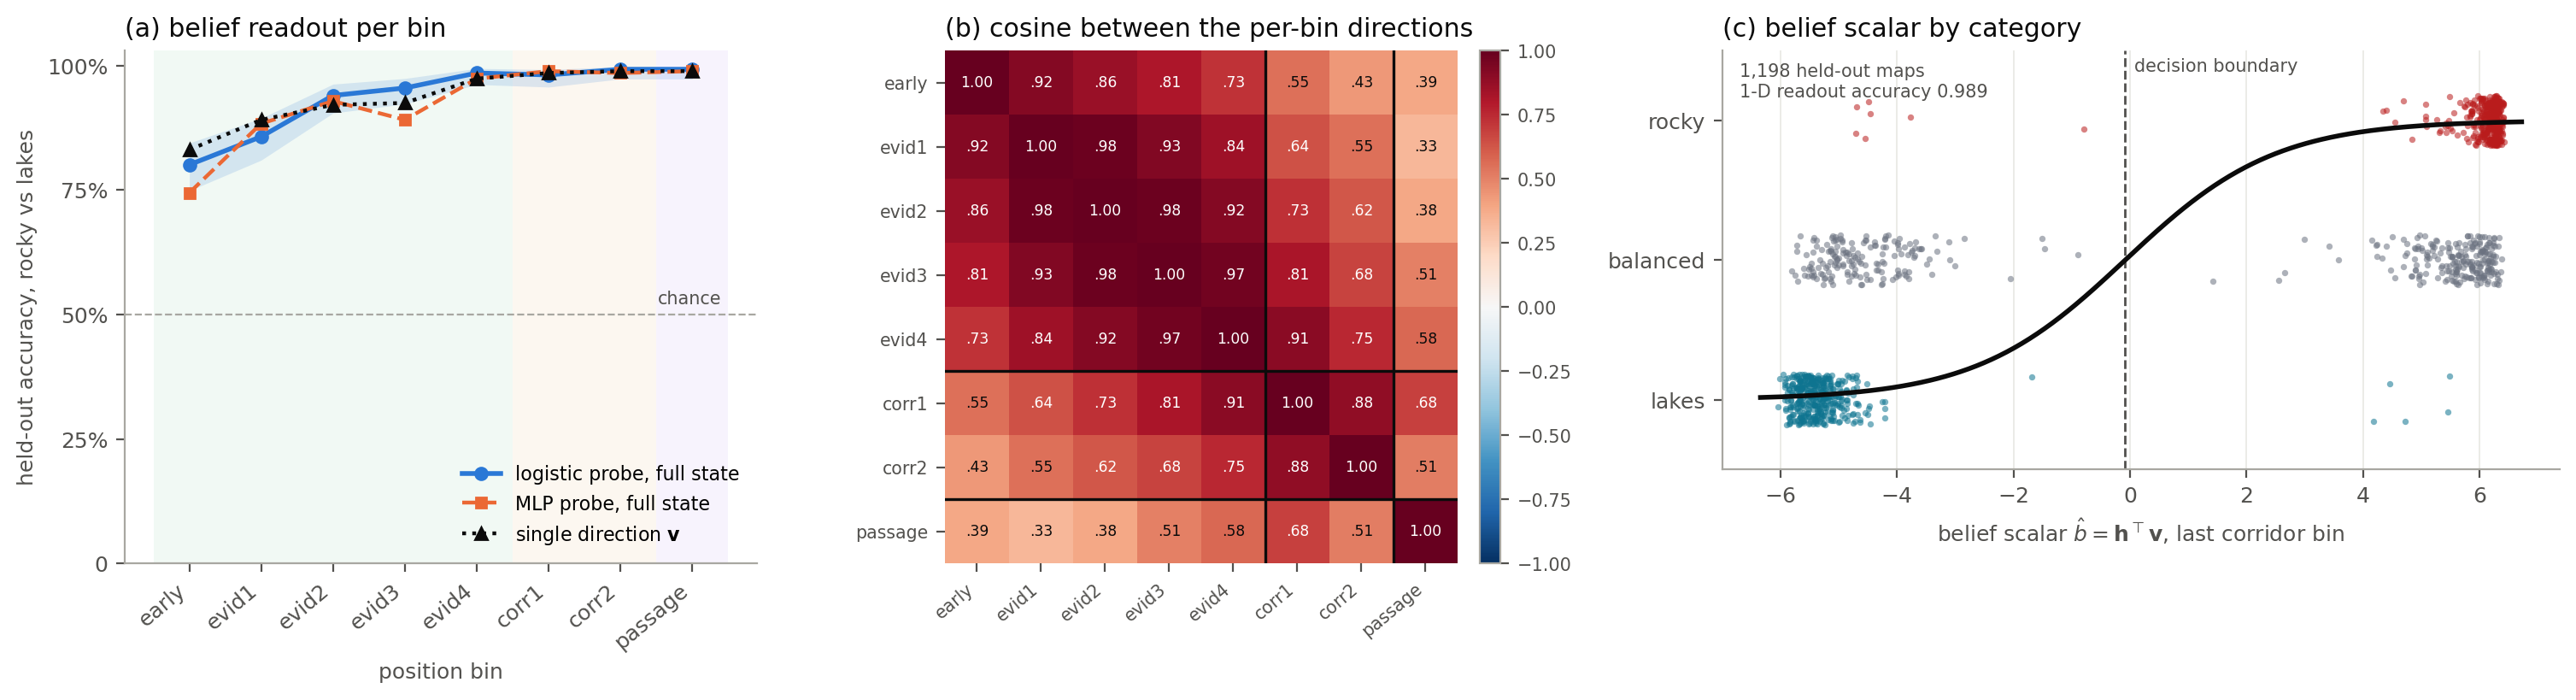
\includegraphics[width=\linewidth]{figures/fig_results_belief.png}
\caption{\textbf{Belief is represented as a single direction} (a) Held-out belief accuracy for rocky against lakes in every position
bin: (i) a logistic-regression probe and (ii) an MLP probe on the full $128$-d state,
and (iii) a logistic regression on the single scalar $b_t=\mathbf{h}_t^{\top}\mathbf{v}$,
where $\mathbf{v}$ is the difference-of-means direction. The scalar matches the full-state probes everywhere, and all three reach
$0.98$ or more from the corridor on. (b) Cosine between the directions $\mathbf{v}$ fitted in different bins.
(c) States projected on the belief direction per map category in bin \textit{corr2}; the curve is the logistic regression on this scalar, with $98.9\%$ held-out accuracy. $57\%$ of balanced maps are classified as rocky.}
\label{fig:results_belief}
\end{figure}

\subsection{The final decision depends on the belief}
\label{sec:res_causal}
Figure~\ref{fig:results_causal} shows which flag the agent chooses as a
function of the steering dose $\alpha$. Pushing the belief of a lakes map
toward rocky smoothly raises the probability of the top flag, until the agent
takes it every time; pushing a rocky map toward lakes does the mirror image.
The response is sigmoidal: small doses do nothing, then the decision flips
over a narrow range of $\alpha$, and by one pole-to-pole distance it has
saturated. On balanced maps, where the unsteered agent has a mild preference
for the top flag, the same write selects either flag on demand. The effect
belongs to the direction and not to the size of the edit: a displacement of
the same size along a random direction leaves the decision where the
unsteered agent put it. The write also costs nothing in navigation. Every
steered episode still reaches a flag, and the episodes are as long as the
unsteered ones. The belief direction is thus a clean handle on a high-level
decision: writing to it changes what the agent decides and nothing about how
it moves.

\begin{figure}[h!]
\centering

\includegraphics[width=0.7\linewidth]{figures/fig_results_causal.png}
\caption{\textbf{The belief direction moves the decision.} One write of
$\mathbf{h}\leftarrow\mathbf{h}\pm\alpha g\mathbf{v}$ at the entry of the last
corridor bin, where $\mathbf{v}$ is fitted, on $100$ held-out maps per
category for $\alpha\in\{0,0.1,\dots,1\}$; the flag taken is recorded, error
bars are one binomial standard deviation, $\alpha=0$ is the unsteered agent.
Lakes maps go from $2\%$ top flag to $100\%$ between $\alpha=0.4$ and $0.8$;
rocky maps from $100\%$ to $0$ between $0.5$ and $0.9$; balanced maps from
$62\%$ top to $100\%$ or to $0$ by $\alpha=0.9$. Dashed grey: the control, a
displacement of the same size $\alpha g$ along a random direction, stays
within $0.02$--$0.04$ on lakes, at $1.00$ on rocky and within $0.62$--$0.67$
on balanced maps. Every steered episode reaches a flag, and episode length
stays within three steps of the unsteered agent's at every dose.}
\label{fig:results_causal}
\end{figure}

\subsection{Behavioral steering corrupts the belief}
\label{sec:res_steer}
We steer the agent on the held-out maps where the unsteered agent uses both
tools at least once, six rollouts per map, and suppress one tool at a time
(Table~\ref{tab:clamp_all}). The behavior changes as intended: the suppressed
tool is used less on most maps, the other tool is barely affected, and the
agent still reaches a flag in nearly all episodes. Walking around a mountain
instead of tunnelling through it is costlier, so timeouts rise a little on
rocky maps, but navigation itself is intact. The intervention is a
gradient-based attack on the action distribution \citep{huang2017adversarial},
and at the action head it does exactly what it is asked.

It also does something it was not asked to do. Suppressing the tool that the
map's category needs moves the belief toward the other category, and the flag
decision follows. A lakes map on which the agent cannot bridge is read as a
rocky map: the belief readout crosses to the rocky side and most episodes end
at the rocky flag, which gives no reward. A rocky map on which the agent
cannot tunnel goes the same way in reverse, with the belief landing on the
boundary and almost half of the episodes at the lakes flag. On balanced maps,
where the reward cannot tell, the free choice is captured almost completely
by whichever tool is suppressed. The effect is one-directional: suppressing
the other tool, tunnelling on lakes maps or bridging on rocky maps, leaves
belief and flag where they were. An edit aimed at a skill lands on the
belief; the two are not separable directions of the hidden state.

\begin{table}[h!]
\centering
\small
\setlength{\tabcolsep}{6pt}
\caption{\textbf{Steering behavior corrupts the belief.} Gated gradient
steering on held-out maps where both tools are used at least once ($138$
balanced, $62$ lakes, $61$ rocky maps; six rollouts each). \emph{\# bridges}
and \emph{\# tunnels} are successful tool uses per episode, the lowest of
each category in bold; \emph{timeout} is the share of episodes that did not
reach a flag; \emph{rocky flag} and \emph{lakes flag} are the agent's
decision; $\hat b(\text{rocky})$ is the mean probability of the rocky category
read from the belief scalar by the logistic probe. Suppressing bridging on
lakes maps raises $\hat b(\text{rocky})$ from $0.03$ to $0.79$ and sends
$74\%$ of episodes to the rocky flag ($1\%$ unsteered); suppressing tunnelling
on rocky maps lowers it from $0.96$ to $0.50$ and sends $43\%$ to the lakes
flag ($4\%$ unsteered). Failure modes in red.}
\label{tab:clamp_all}
\begin{tabular}{@{}llrrrrrr@{}}
\toprule
& & & & \multicolumn{3}{c}{share of episodes} & \\
\cmidrule(lr){5-7}
Category & Regime & \# bridges & \# tunnels & timeout & rocky flag & lakes flag & $\hat b(\text{rocky})$ \\
\midrule
balanced & unsteered & 4.21 & 4.94 & 0.00 & 0.60 & 0.40 & 0.61 \\
 & suppress bridge & \textbf{2.61} & 4.79 & 0.01 & 0.97 & 0.02 & 0.97 \\
 & suppress tunnel & 4.12 & \textbf{3.83} & 0.06 & 0.19 & 0.75 & 0.23 \\
\midrule
lakes & unsteered & 6.04 & 1.92 & 0.00 & 0.01 & 0.99 & 0.03 \\
 & suppress bridge & \textbf{4.66} & 1.94 & 0.05 & \textcolor{red}{\textbf{0.74}} & 0.22 & 0.79 \\
 & suppress tunnel & 6.25 & \textbf{1.31} & 0.00 & 0.00 & 1.00 & 0.02 \\
\midrule
rocky & unsteered & 1.98 & 6.86 & 0.00 & 0.96 & 0.04 & 0.96 \\
 & suppress bridge & \textbf{0.96} & 7.03 & 0.00 & 1.00 & 0.00 & 0.99 \\
 & suppress tunnel & 2.02 & \textbf{5.42} & 0.14 & 0.43 & \textcolor{red}{\textbf{0.43}} & 0.50 \\
\bottomrule
\end{tabular}
\end{table}

